\subsection{Your site should look good}

It is important that the information is attractive, eye-catching and with sparkle. This is not only important from a conceptual point of view, but also from a functional one. We saw this previously, where we considered the importance
of good data presentation, using a structure that guides the user in a logical and orderly manner.\\

We want to grab the users attention from the outset. For this we propose the following desirable features for the tool- that it be fun, entertaining,
modern, current, easy to use, high quality, attractive and beautiful. Although some of these characteristics are subjective, there are techniques available to achieve these objectives.\\

Other more technical characteristics are: \\

\textbf{Consistency.} Controls that perform similar actions must maintain the same design. Functionalities
should also follow this principle. \\

\textbf{Cleaning and order.} An organized design looks better, give a more peaceful feeling and enables the user to find what they are looking for
more easily.\\

\textbf{Details.} A label with different typology or other color may jarr the user's perception. Only use when
we want to highlight something in particular!. \\

\textbf{Sena de identidad.} It is highly recommended to 'brand' ourselves, so that users can recognize us quickly. For this we can utilize a symbol, a combination of colors, a logo, etc.\\

To be able to hook our users, gamification is currently widely used. This is where we give a gaming aspect to the representation of the data. The user tries it because it catches their attention, it's fun.
Certainly, at some point the novelty wears off, but, even so, the user has learned to use the interface and now feels well-disposed to continue to use it.

\subsubsection*{Suggested strategies}

To make an attractive design, we must keep abreast of current trends, as well as study good design practices.
It is highly recommended to maintain a simple and clean design, to use standards and mechanisms that are familiar to users,
to care of details and to present our identity.

\subsubsection*{In the context of Aire Guru \ldots}

As we commented previously the design has been based on Google's Material Design, using straight lines, differentiating individual sections by using rectangles and using colors that contrast the information from the background.
The background color for the graphics is a neutral white. Only shades of blue, gray and white are used. In addition, we have chosen a font that is easy to read.\\

The sections are arranged neatly and structured by using a header and a body.\\

The central page consists of a header, the body and a footer. Both the header and the footer are static,
they are shown in all the pages and they contain all the information needed to navigate between pages.
The body is divided into three horizontal sections, the upper area with the map and the general information about the selected point,
the central area where we can filter the pollutants by medical conditions and information about the current air status, and the
lower area where we will find the zone and custom history.

\begin{figure}[ht]
    \centering
    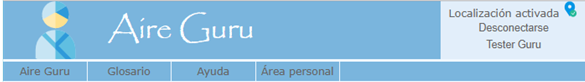
\includegraphics[width=12cm]{heading}
    \caption{Heading}
\end{figure}
 
    The symbol of our webtool is a genius, is a guru. We also include "Aire" in the logo, because it perfectly represents 
    what we show with our webtool. Aire Guru is the genius of air.
    
    Finally, we've taken into account that the user may wish to use our webtool on different devices. We've implemented
    two different formats, one for larger screens such as the computer and another for smaller format tablets or mobiles.

\subsubsection*{Evaluation}  

\begin{itemize}
    \done The design is organized and clean. 
    \done The user can find easierly what he is looking for.
    \done Minimized numbers of clicks since the most relevant info is shown directly in the launching page.
    \crossed Although there have been attempts to implement the design aesthetics that are now trending on the market, the design can be improved.
\end{itemize}